%\documentclass[handout]{beamer}
\documentclass[10pt,appendixnumberbeamer]{beamer}
%\usepackage{handoutWithNotes}
%\pgfpagesuselayout{4 on 1 with notes}[a4paper,border shrink=5mm]
%\pgfpagesuselayout{1 on 1 with notes landscape}[a4paper,border shrink=5mm]
\usetheme[
  outer/progressbar=foot,
%outer/numbering=fraction,
]{metropolis}
\usepackage{amsmath, amssymb, amsthm, mathtools,media9}
\usepackage[export]{adjustbox}

\usepackage[default]{sourcesanspro}
\usepackage[utf8]{inputenc}
\usepackage[T1]{fontenc}
\metroset{titleformat=smallcaps}

\usepackage{tikz}
\usetikzlibrary{mindmap,shadows}
\usepackage{animate}
\usepackage[compatibility=false]{caption}

\usepackage{algorithm}
\usepackage{algorithmic}
\usepackage{bm}

\usepackage{listings}
\usepackage{tcolorbox}

\newcommand{\lstfont}[1]{\color{#1}\scriptsize\ttfamily}

\lstset { %
    language=[ANSI]C++,
    backgroundcolor=\color{black!5}, % set backgroundcolor
    basicstyle=\scriptsize,% basic font setting
    showstringspaces=false,
    breaklines=true,
}


\usepackage{graphicx,subfigure}
\usetikzlibrary{spy,calc,patterns,arrows,decorations.pathmorphing,backgrounds,positioning,fit,petri,mindmap,trees,intersections}
\usepackage{keystroke}
\usepackage{color}
\usepackage{multicol}
%\usepackage{multimedia}
\usepackage{enumerate}
\usepackage{multirow}
\usepackage{pgfplots,tikz,tcolorbox}
%\usepackage{appendixnumberbeamer}

%\setbeamertemplate{frame footer}{My custom footer}

\pgfplotsset{compat=newest}

%\expandafter\def\expandafter\insertshorttitle\expandafter{%
 % \insertshorttitle\hfill\insertframenumber\,/\,\inserttotalframenumber}
%\usepackage{enumitem}


%\usepackage[T1]{fontenc}
\usepackage{color,hyperref}
\definecolor{darkblue}{rgb}{0.0,0.0,0.5}
%\hypersetup{colorlinks,breaklinks,
%            linkcolor=darkblue,urlcolor=darkblue,
%            anchorcolor=darkblue,citecolor=darkblue}
\usetikzlibrary{patterns}
\usetikzlibrary{decorations.pathmorphing,backgrounds,positioning,fit,petri,mindmap,trees}
\usepgflibrary{arrows,shapes.geometric}
\usepgflibrary{shapes.symbols}
%\hypersetup{colorlinks,breaklinks,linkcolor=darkblue,urlcolor=darkblue,anchorcolor=darkblue,citecolor=darkblue}
\usetikzlibrary{spy,calc,patterns,arrows,decorations.pathmorphing,backgrounds,positioning,fit,petri,mindmap,trees,intersections}
\usepackage{color}
\usepackage{multirow}
\usetikzlibrary{arrows,positioning} 
\tikzset{
    %Define standard arrow tip
    >=stealth',
    %Define style for boxes
    punkt/.style={
           rectangle,
           rounded corners,
           draw=black, very thick,
           text width=8.5em,
           minimum height=2em,
           text centered},
    % Define arrow style
    pil/.style={
           ->,
           thick,
           shorten <=2pt,
           shorten >=2pt,}
}

%\usepackage[hang]{footmisc}
%\setlength\footnotemargin{10pt}

\setbeamertemplate{caption}[numbered]
\usepgfplotslibrary{statistics}

\usetikzlibrary{fadings}
\tikzfading[name=fade out,
  inner color=transparent!0, outer color=transparent!100]


%\setbeameroption{show notes}
%\setbeameroption{show only notes}


\newcommand{\network}[1]{
\begin{figure}[h]
\centering
\begin{tikzpicture}[scale = 0.75,-,draw=black!50, node distance=\layersep]
    \tikzstyle{neuron}=[circle,fill=black!25,minimum size=17pt,inner sep=0pt];
    \tikzstyle{unit}=[neuron, fill=red!50];
    \tikzstyle{spike}=[neuron, fill=blue!50];
 \def \radius {2cm}
% \def \margin {8}
 \def \n {6}
 \foreach \s in {1,...,\n}
  \node[unit] (\s) at ({360/\n * (\s - 1) - 180}:\radius) {$\s$};
 \foreach \s in {1,...,\n}
  \foreach \t in {\s,...,\n}
   \draw (\t) -- (\s);
 \foreach \s in {1,...,\n}
   \draw[very thick] (#1) -- (\s);
   \node[spike] (#1) at ({360/\n * (#1 - 1) - 180}:\radius) {};
\end{tikzpicture}
\end{figure}

}


\newcommand{\networkwc}[6]{
\begin{figure}[h]
\centering
\begin{tikzpicture}[scale = 1,-,draw=black!50, node distance=\layersep]
    \tikzstyle{neuron}=[circle,fill=black!25,minimum size=17pt,inner sep=0pt];
    \tikzstyle{unit}=[neuron, fill=red!50];
    \tikzstyle{spike}=[neuron, fill=blue!50];
 \def \radius {2cm}
% \def \margin {8}
 \def \n {6}
% \foreach \s in {1,...,\n}
  \node[unit] (1) at (- 180:\radius) {{\color{white}#1}};
   \node[unit] (2) at (- 120:\radius) {{\color{white}#2}};
     \node[unit] (3) at (- 60:\radius) {{\color{white}#3}};
   \node[unit] (4) at (0:\radius) {{\color{white}#4}};
  \node[unit] (5) at (60:\radius) {{\color{white}#5}};
   \node[unit] (6) at (120:\radius) {{\color{white}#6}};
 \foreach \s in {1,...,\n}
  \foreach \t in {\s,...,\n}
   \draw (\t) -- (\s);
% \foreach \s in {1,...,\n}
%   \draw[very thick] (#1) -- (\s);
%   \node[spike] (#1) at ({360/\n * (#1 - 1) - 180}:\radius) {};
\end{tikzpicture}
\end{figure}
}

\newcommand{\networkwcww}[6]{
\begin{figure}[h]
\centering
\begin{tikzpicture}[scale = 1,-,draw=black!50, node distance=\layersep]
    \tikzstyle{neuron}=[circle,fill=black!25,minimum size=17pt,inner sep=0pt];
    \tikzstyle{unit}=[neuron, fill=red!50];
    \tikzstyle{spike}=[neuron, fill=blue!50];
 \def \radius {2cm}
% \def \margin {8}
 \def \n {6}
% \foreach \s in {1,...,\n}
  \node[unit] (1) at (- 180:\radius) {{\color{white}#1}};
   \node[unit] (2) at (- 120:\radius) {{\color{white}#2}};
     \node[unit] (3) at (- 60:\radius) {{\color{white}#3}};
   \node[unit] (4) at (0:\radius) {{\color{white}#4}};
  \node[unit] (5) at (60:\radius) {{\color{white}#5}};
   \node[unit] (6) at (120:\radius) {{\color{white}#6}};
 \draw (1) edge node[below left] {\small $-1$} (2);
 \draw (2) edge node[below] {\small $-3$} (3);
  \draw (3) edge node[below right] {\small $-1$} (4);
   \draw (4) edge node[above right] {\small $3$} (5);
    \draw (5) edge node[above] {\small $-2$} (6);
         \draw (6) edge node[above left] {\small $3$} (1);
     \draw (2) edge node[right] {\small $2$} (6);
      \draw (3) edge node[left] {\small $3$} (5);
%  \draw (i) edge node[right] {\small $W_{ij} = W_{ji}$} (j);

 % \foreach \s in {1,...,\n}
%   \draw[very thick] (#1) -- (\s);
%   \node[spike] (#1) at ({360/\n * (#1 - 1) - 180}:\radius) {};
\end{tikzpicture}
\end{figure}
}

\newcommand{\mpm}[6]{
\begin{figure}[h]
\centering
\begin{tikzpicture}[scale = 1,-,draw=black!50, node distance=\layersep,>=stealth]
    \tikzstyle{neuron}=[circle,fill=black!25,minimum size=17pt,inner sep=0pt];
    \tikzstyle{unit}=[neuron, fill=red!50,thick];
 \def \radius {2cm}
% \def \margin {8}
 \def \n {6}
 \foreach \s in {1,...,\n}{
  \node[unit] (\s) at ({360/\n * (\s - 1) - 180}:\radius) {};
%  \node (S-\s) at ($(\s) + {360/\n * (\s - 1) - 180}:5mm$) {$s_i$};
}  

   \DoubleLine{1}{2}{<-,draw=black!50}{}{->,draw=black!50}{};
   \DoubleLine{1}{3}{<-,draw=black!50}{}{->,draw=black!50}{};
   \DoubleLine{1}{4}{<-,draw=black!50}{}{->,draw=black!50}{};
   \DoubleLine{1}{5}{<-,draw=black!50}{}{->,draw=black!50}{};
   \DoubleLine{1}{6}{<-,draw=black!50}{}{->,draw=black!50}{};
    \DoubleLine{2}{3}{<-,draw=black!50}{}{->,draw=black!50}{};
   \DoubleLine{2}{4}{<-,draw=black!50}{}{->,draw=black!50}{};
   \DoubleLine{2}{5}{<-,draw=black!50}{}{->,draw=black!50}{};
   \DoubleLine{2}{6}{<-,draw=black!50}{}{->,draw=black!50}{};
   \DoubleLine{3}{4}{<-,draw=black!50}{}{->,draw=black!50}{};
   \DoubleLine{3}{5}{<-,draw=black!50}{}{->,draw=black!50}{};
   \DoubleLine{3}{6}{<-,draw=black!50}{}{->,draw=black!50}{};
    \DoubleLine{4}{5}{<-,draw=black!50}{}{->,draw=black!50}{};
   \DoubleLine{4}{6}{<-,draw=black!50}{}{->,draw=black!50}{};
   \DoubleLine{5}{6}{<-,draw=black!50}{}{->,draw=black!50}{};

   \node[unit] (1) at (- 180:\radius) {{\color{white}#1}};
   \node[unit] (2) at (- 120:\radius) {{\color{white}#2}};
     \node[unit] (3) at (- 60:\radius) {{\color{white}#3}};
   \node[unit] (4) at (0:\radius) {{\color{white}#4}};
  \node[unit] (5) at (60:\radius) {{\color{white}#5}};
   \node[unit] (6) at (120:\radius) {{\color{white}#6}};
%   \draw[color=None] (i) edge node[right] {\small $W_{ij}$} (j);
%   \draw[color=None] (i) edge node[left] {\small $W_{ij}$} (j);
\end{tikzpicture}
\end{figure}

}

\newcommand\DoubleLine[7][1pt]{%
    \path(#2)--(#3)coordinate[at start](h1)coordinate[at end](h2);
    \draw[#4]($(h1)!#1!90:(h2)$)-- node [left=-.75mm] {#5} ($(h2)!#1!-90:(h1)$); 
    \draw[#6]($(h1)!#1!-90:(h2)$)-- node [right=-.75mm] {#7} ($(h2)!#1!90:(h1)$);
    }

\tikzstyle{innergrid}=[gray!80]
\tikzstyle{tile}=[green!60!black, thick]
\tikzstyle{sync}=[red!60!black, thick, dashed]
\tikzstyle{thread}=[->, decorate, decoration={snake, amplitude=.6}]
\tikzstyle{examplecell}=[fill=orange, opacity=.5]
\tikzstyle{kernelcall}=[#1, rounded corners=2pt, very thick, pattern color=#1]
\tikzstyle{kernelarrow}=[->, thick, out=90, in=180]
\tikzstyle{imglabel}=[anchor=west, text opacity=1.0, fill=white, fill opacity=.5,
                      text height=1ex, text depth=.25ex, rounded corners]

%\newcommand\drawthread[4]{%
%  \pgfmathsetmacro{\ybot}{(1 + \nrblockbodies) * #2}
%  \draw [#1] (0.5, \ybot + 0.5 + #3) -- ++(#4 - 1, 0);%
%}

\newcommand\drawthread[4]{%
  \pgfmathsetmacro{\ybot}{(1 + \nrblockbodies) * #2}
  \draw [#1,<-] ( 0.5 + #3,\ybot +1) -- ++(0,#4 - 1);%
}

\def\dogcoordinates{ ( 3.666,15.100) 
( 2.833,14.900) ( 2.233,14.366) ( 2.133,13.966)  
( 1.733,13.966) ( 1.433,13.366) ( 1.433,13.000)  
( 1.566,12.633) ( 2.066,12.333) ( 2.466,12.200)  
( 2.766,12.200) ( 3.000,12.333) ( 3.333,12.300)
( 3.533,12.033) ( 3.666,11.400) ( 4.033,10.566) 
( 4.000, 9.133) ( 4.833, 7.300) ( 5.300, 4.400)  
( 5.333, 3.400) ( 5.233, 2.700) ( 4.700, 2.466)
( 4.633, 2.100) ( 5.133, 1.933) ( 5.600, 1.933) 
( 5.833, 2.033) ( 6.033, 2.333) ( 6.166, 3.166)
( 6.300, 3.300) ( 6.366, 5.366) ( 6.566, 6.966)  
( 8.233, 7.133) (11.033, 8.033) (11.600, 7.733) 
(12.266, 6.600) (13.300, 5.500) (14.066, 4.933)  
(14.600, 4.300) (14.733, 3.966) (14.700, 2.866) 
(14.600, 2.666) (14.233, 2.466) (14.166, 2.066)  
(14.333, 1.933) (14.666, 1.900) (15.133, 1.966)  
(15.400, 2.200) (15.733, 4.833) (15.333, 5.400) 
(14.600, 6.100) (14.266, 7.033) (14.000, 9.800)  
(13.833,10.433) (13.666,10.666) (14.033,11.366)  
(14.033,11.633) (13.666,11.666) (13.200,11.200)  
(12.100,11.433) (10.400,11.400) ( 8.366,11.533)  
( 7.966,11.833) ( 7.233,11.966) ( 6.966,12.200) 
( 6.666,12.233) ( 5.700,13.600) ( 4.966,14.266) 
( 4.933,14.533) ( 4.733,14.733) ( 4.366,14.900)  
( 4.300,15.033) ( 3.700,15.100) }


\makeatletter
\newif\iftikztransformnodecoordinates
\tikzset{transform node coordinates/.is if=tikztransformnodecoordinates}


\def\tikz@parse@node#1(#2){%
    \pgfutil@in@.{#2}%
    \ifpgfutil@in@
        \tikz@calc@anchor#2\tikz@stop%
    \else%
        \tikz@calc@anchor#2.center\tikz@stop%
        \expandafter\ifx\csname pgf@sh@ns@#2\endcsname\tikz@coordinate@text%
        \else
            \tikz@shapebordertrue%
            \def\tikz@shapeborder@name{#2}%
        \fi%
    \fi%
    \iftikztransformnodecoordinates%
        \pgf@pos@transform{\pgf@x}{\pgf@y}%
    \fi
    \edef\tikz@marshal{\noexpand#1{\noexpand\pgfqpoint{\the\pgf@x}{\the\pgf@y}}}%
    \tikz@marshal%
}

\title{Simulating Recurrent Neural Networks on Graphic Processing Units}
\subtitle{Summer Project}
%\institute{SUTD}
\author{Zhangsheng Lai}
%\date{\today}



\pgfmathdeclarefunction{gauss}{2}{%
  \pgfmathparse{1/(#2*sqrt(2*pi))*exp(-((x-#1)^2)/(2*#2^2))}%
}
%\pgfmathdeclarefunction{gauss1}{2}{%
  %\pgfmathparse{(1/(#2*sqrt(2*pi))*exp(-((-x-#1)^2)/(2*#2^2)))*exp(-x)}%
%}
\pgfmathdeclarefunction{gauss2}{2}{%
  \pgfmathparse{(1/(#2*sqrt(2*pi))*exp(-0.5*abs(x)-#1)*(sqrt(abs(x)))}%
}

%\pgfmathdeclarefunction{gauss2}{2}{%
  %\pgfmathparse{(1/(#2*sqrt(2*pi))*exp(-((x-#1)^2)/(2*#2^2)))*exp(x)}%
%}
\pgfmathdeclarefunction{gauss1}{2}{%
  \pgfmathparse{(1/(#2*sqrt(2*pi))*exp(-0.5*x-#1)*(sqrt(x))}%
}
\def\checkmark{\tikz\fill[scale=0.4](0,.35) -- (.25,0) -- (1,.7) -- (.25,.15) -- cycle;}

\newcommand*{\Perm}[2]{{}^{#1}\!P_{#2}}%
\newcommand*{\Comb}[2]{{}^{#1}C_{#2}}%
\begin{document}


\begin{frame}
\titlepage
\end{frame}


%\begin{frame}{Contents}
%\tableofcontents
%\end{frame}

\section{Introduction}

\begin{frame}{Introduction}
\begin{figure}[h]
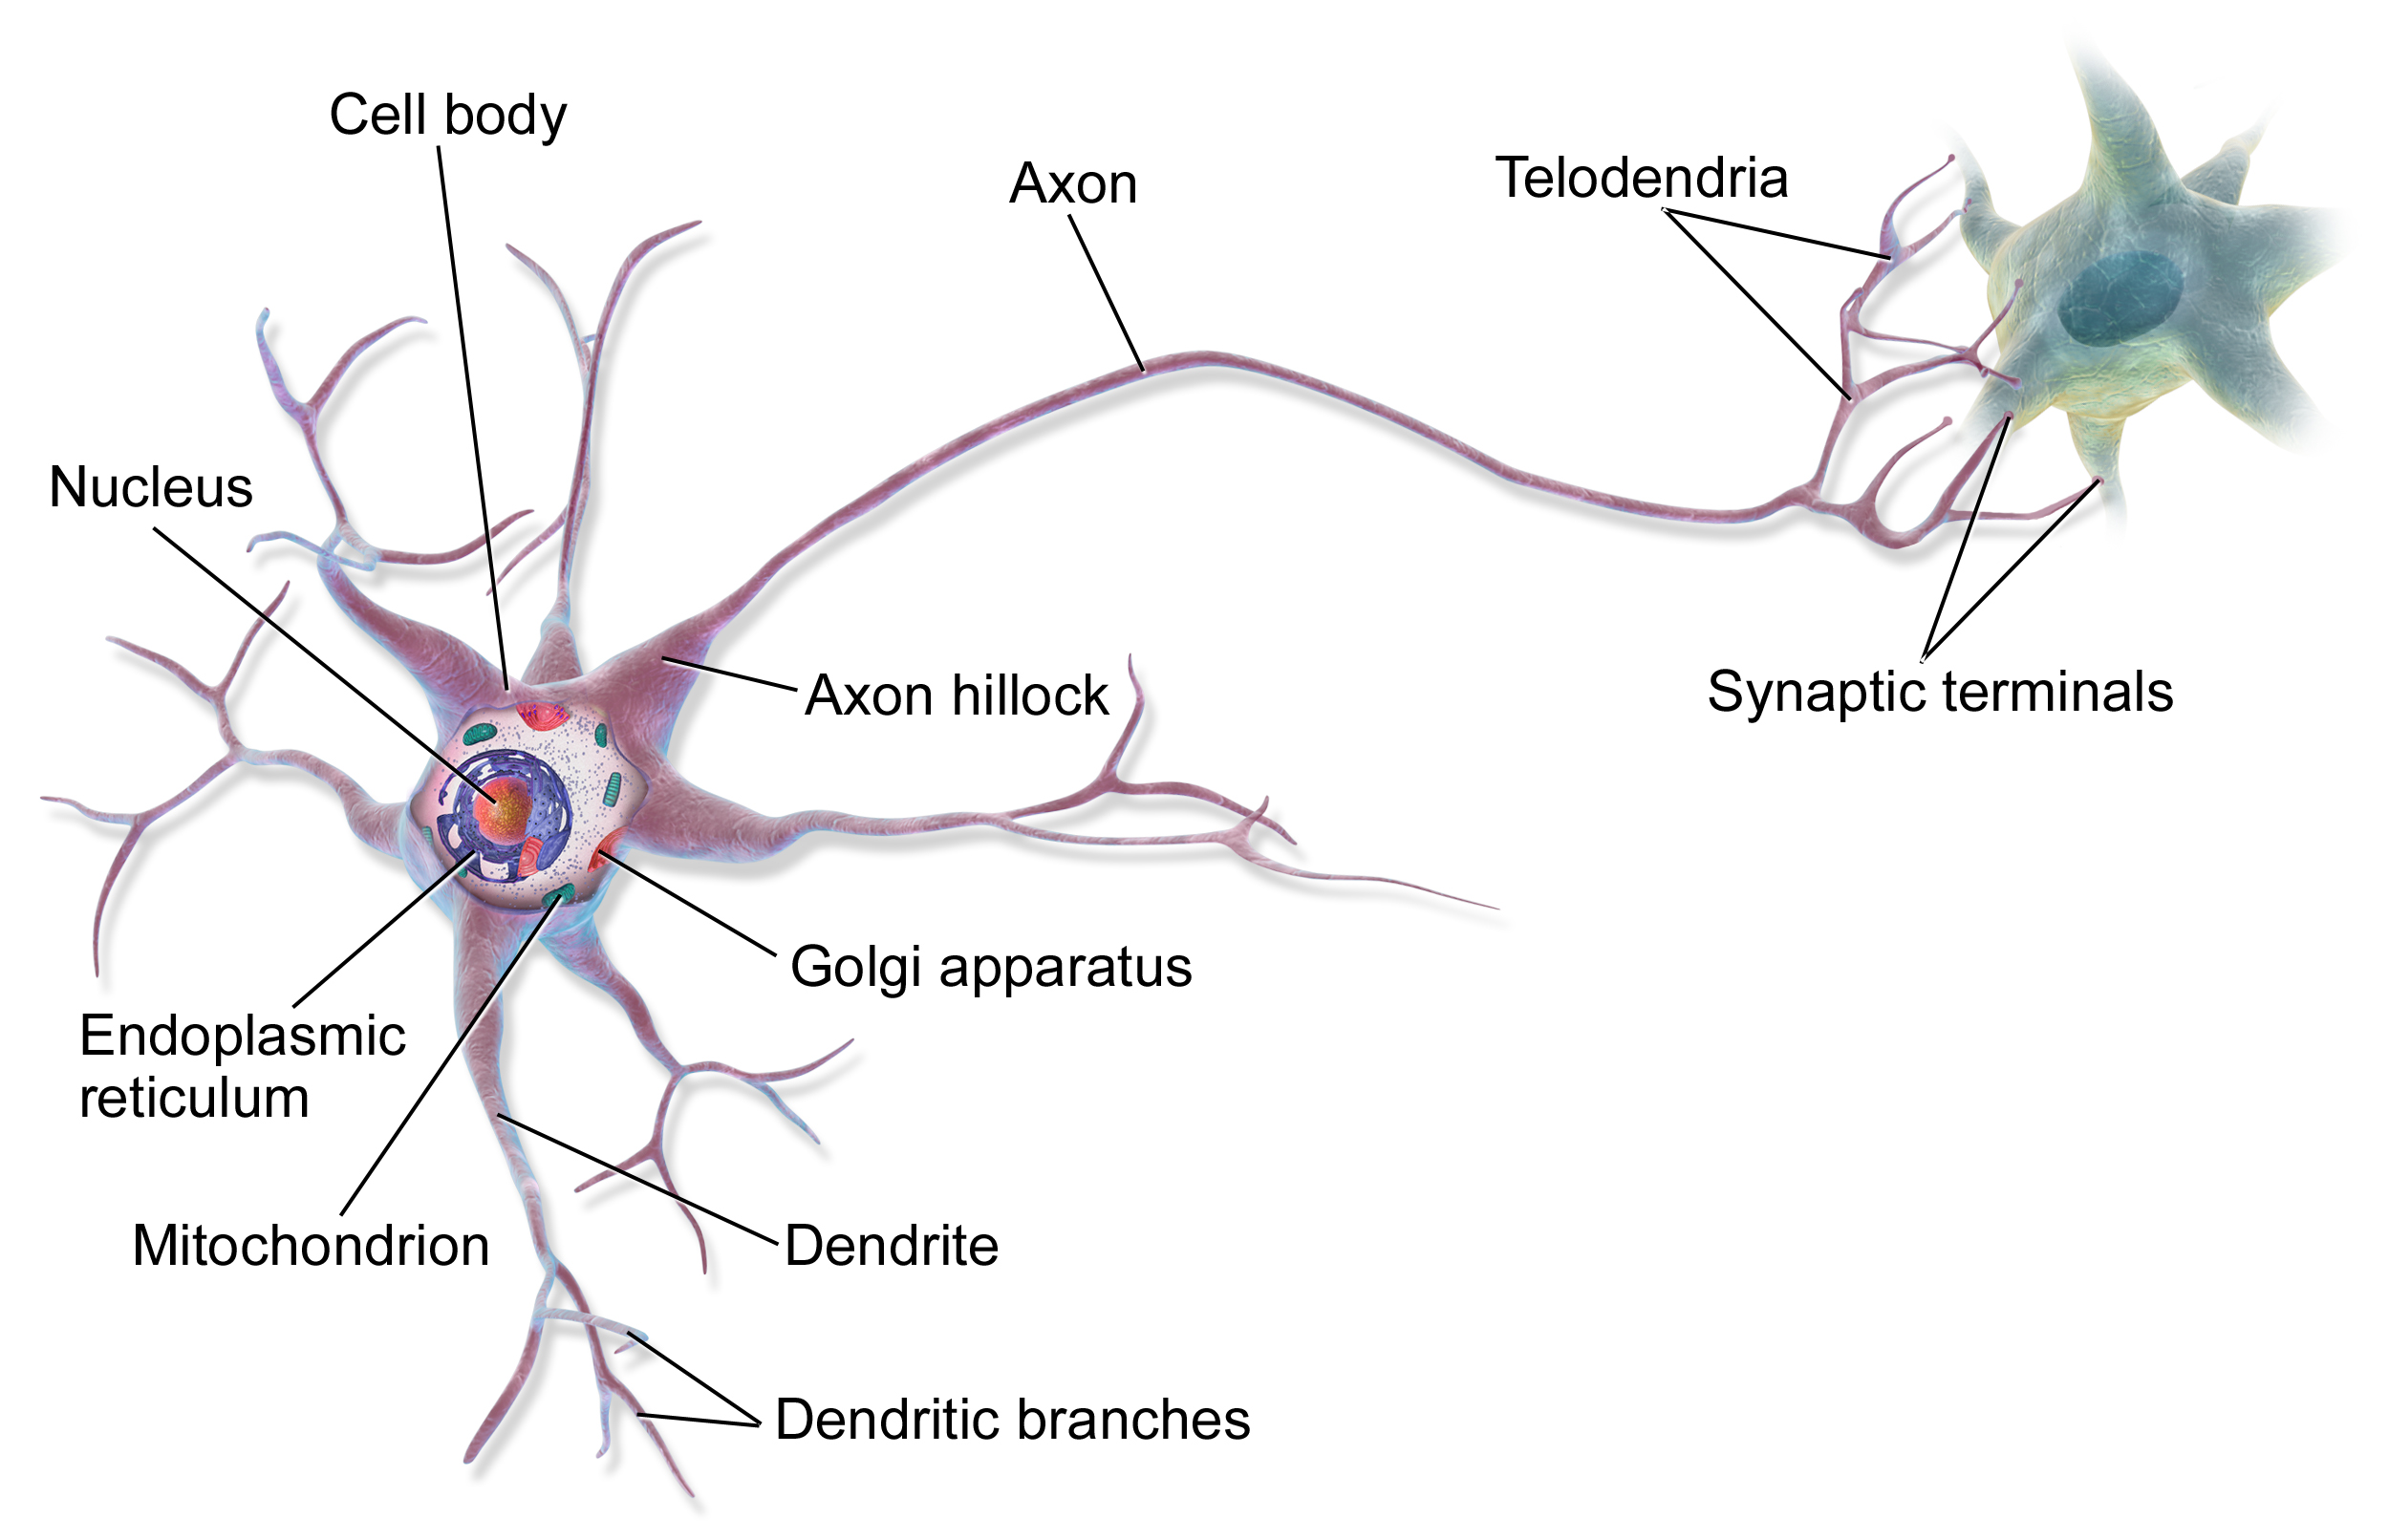
\includegraphics[scale=0.1]{Blausen_0657_MultipolarNeuron.png}
\caption{Anatomy of a neuron\footnote{By BruceBlaus - Own work, CC BY 3.0, https://commons.wikimedia.org/w/index.php?curid=28761830}}
\note{
\scriptsize
\begin{itemize}
\item the features that define a neuron are electrical excitability, where a neuron spikes and discharge electrical signals through the synapses, which are complex membrane junctions that transmit signals to other neurons
\item there are approximately $10^{14}$ neurons in the human brain
\item artifical neuron networks are inspired by these biological neurons 
\end{itemize}
}
\end{figure}


\end{frame}


%\begin{frame}{Introduction}
%\begin{definition}
%A \alert{feedforward neural network} is an artificial neural network where connections between the units do not form a cycle.
%\end{definition}
%
%\begin{definition}
%A \alert{recurrent neural network} is an artificial neural network where connections between units form a directed cycle.
%\end{definition}

%\end{frame}

\begin{frame}{Feedforward Neural Network}
\begin{figure}[h]
\centering

\def\layersep{1.8cm}

\begin{tikzpicture}[scale = 1,draw=black!50, node distance=\layersep]
%    \tikzstyle{every pin edge}=[<-,shorten <=1pt]
    \tikzstyle{neuron}=[circle,fill=black!25,minimum size=10pt,inner sep=0pt]
    \tikzstyle{input neuron}=[neuron, fill=blue!70!red!70];
        \tikzstyle{hidden neuron 0}=[neuron, fill=blue!50!red!50];
    \tikzstyle{hidden neuron 1}=[neuron, fill=red!80];
    \tikzstyle{hidden neuron 2}=[neuron, fill=red!50];
        \tikzstyle{output neuron}=[neuron, fill=orange!70];

    \tikzstyle{annot} = [text width=4em, text centered]

    % Draw the input layer nodes
    \foreach \name / \y in {1,...,6}
    	\node[input neuron] (I-\name) at (0,-\y) {};
		\node[input neuron] (I-4) at (0,-4) {};

 \foreach \name / \y in {1,...,6}
    	            \node[hidden neuron 0] (B-\name) at (\layersep,-\y cm) {};


    % Draw the hidden layer nodes
    \foreach \name / \y in {1,...,6}
            \node[hidden neuron 1] (H-\name) at (2*\layersep,-\y cm) {};
    % Draw the output layer node
%    \node[output neuron,pin={[pin edge={->}]right:$h_{W,b}(x) = f(z_{1}^{(3)}) = a_{1}^{(3)}$}, right of=H-3] (O) {};
 \foreach \name / \y in {1,...,6}
            \node[hidden neuron 2] (P-\name) at (3*\layersep,-\y cm) {};

 \foreach \name / \y in {1,...,3}
 \path[yshift=-1.5cm]
      node[output neuron] (O-\name) at (4*\layersep,-\y cm) {};

    % Connect every node in the input layer with every node in the
    % hidden layer.
    \foreach \source in {1,...,6}
        \foreach \dest in {1,...,6}
            \path[color = blue!70!red!70] (I-\source) edge (B-\dest);

  \foreach \source in {1,...,6}
        \foreach \dest in {1,...,6}
            \path[color = blue!50!red!50] (B-\source) edge (H-\dest);

\foreach \source in {1,...,6}
        \foreach \dest in {1,...,6}
            \path[color = red!80] (H-\source) edge (P-\dest);

\foreach \source in {1,...,6}
        \foreach \dest in {1,...,3}
            \path[color = red!50] (P-\source) edge (O-\dest);

    \node[annot,below=0.25cm of {H-6}, node distance=1cm] (hl2) {\small {\color{red!80}L3}};
    \node[annot,left of ={hl2}](hl1) {\small {\color{blue!50!red!50}L2}};
        \node[annot,left of=hl1] {\small {\color{blue!70!red!70}L1}};
            \node[annot,right of=hl2](hl3) {\small {\color{red!50}L4}};
            \node[annot,right of=hl3] {\small {\color{orange!70}L5}};
\node[left=1.25cm of {I-3},yshift=-.5cm] (dog) {};
 \foreach \dest in {1,...,6}
            \draw[color = black!30,->,>=stealth, decoration, decoration={snake}] (dog) -- (I-\dest);

            \filldraw [black!50,scale=0.1,transform node coordinates,shift={(-25,-45)}]
  plot  coordinates \dogcoordinates  -- cycle;
  
%  \node[output neuron] at (O-2) {{\color{white}1}};
%    \node[hidden neuron 0] at (B-2) {{\color{white}1}};
%        \node[hidden neuron 1] at (H-4) {{\color{white}1}};
%            \node[hidden neuron 2] at (P-6) {{\color{white}1}};
%             \node[input neuron] at (I-4) {{\color{white}1}};
             \path[color = blue!70!red!70, very thick] (I-4) edge (B-2);
           \path[color = blue!50!red!50, very thick] (B-2) edge (H-4);
            \path[color = red!80, very thick] (H-4) edge (P-6);
      \path[color = red!50, very thick] (P-6) edge (O-2);
      \node[right=0.25cm of {O-2}](w) {{\color{orange!70}``Dog''}};
            \draw[->,>=stealth, color=orange!70,very thick] (O-2) -- (w);
\end{tikzpicture}
\caption{Feedforward Neural Network}
\label{fig:feedforwardnn}
\end{figure}
\end{frame}

\note{
\scriptsize
\begin{itemize}
\item for example we have feedforward neural networks where connections between the units do not form a cycle
\item we have managed to use feedforward neural networks, to classify images very well
\item however the connections between the neurons in our brain are much more complex than those in the feedforward neural networks
\item however, the methodology used to do classification is based on learning parameters of the model and then do matrix multiplication to obtain a probability of it being classified as a particular class.
%\item supervised: MNIST digits classification, unsupervised: autoencoders
%\item these neural networks are the more popular and mainstream ones, but today we are going to look at RNNs and how to simulate them.
%\item we will look at some RNNs where their architecture is closer to our brains and by building such neural networks with the neurons matching the number of neurons in the brain, we hope to possibly arrive at some learning theories that is close to how learning is done in the brain, if not as good as the brain
%\item to construct such a big network of neurons, we have to rely on hardware that are more suitable to dealing with large numbers of computation, thus we would want to simulate these RNNs on GPUs
\end{itemize}
}



%\note{
%\scriptsize
%\begin{itemize}
%\item for feedforward neural networks, we have can have supervised or unsupervised
%\item supervised: MNIST digits classification, unsupervised: autoencoders
%\item these neural networks are the more popular and mainstream ones, but today we are going to look at RNNs and how to simulate them.
%\item we will look at some RNNs and discrete time steps and then look at one with continuous time steps.
%\end{itemize}
%}

\section{Recurrent Neural Networks}



\note{
\scriptsize
\begin{itemize}
\item recurrent neural networks are artificial neural network where connections between units form a directed cycle.
\item these neural networks are the more popular and mainstream ones, but today we are going to look at RNNs and how to simulate them.
\item one of the more popular RNN is Long short term memory (LSTM), and they are able to connect previous information to the present task, such as using previous video frames might inform the understanding of the present frame, but the neurons in LSTMs communicate with real values, which is different from the way neurons communicate in our brain
\item we will look at some RNNs where their architecture is closer to our brains and by building such neural networks with the neurons matching the number of neurons in the brain, we hope to possibly arrive at some learning theories that is close to how learning is done in the brain, if not as good as the brain
\item to construct such a big network of neurons, we have to rely on hardware that are more suitable to dealing with large numbers of computation, thus we would want to simulate these RNNs on GPUs

\item today I'm going to talk about 2 types of RNNs, Boltzmann machines and McCulloch-Pitts machines
\item their main differences is BM is discrete time and MPM is continuous time, their similarities is that they both have the spiking characteristic in them when we simulate these machines
\end{itemize}
}




\begin{frame}{Boltzmann Machines}
\networkwc{1}{0}{1}{1}{0}{1}
\end{frame}

\note{\scriptsize
\begin{itemize}
\item composed of primitive computing elements called units
\item units has two states, on or off, represented by $\{1,0\}$
\item connected to each other by bi-directional links
\item weights can take on any real value
\item a unit being on or off is taken to mean that the system currently accepts or rejects some elemental hypothesis of the domain
\item weight on a link represents a weak pairwise constrain between two hypothesis
\item positive (negative) weights indicate that two hypothesis support (contradict) one another with other things being equal
\item link weights are symmetric, having the same strength in both directions
%\item adopts these states as a function of the states of its neighbouring units and weights of its links to them, it is a probabilistic function for a Boltzmann machine.

\end{itemize}
}





\begin{frame}{Boltzmann Machines}
\begin{figure}[h]
\centering
\begin{tikzpicture}[scale = 1,-,draw=black!50, node distance=\layersep]
    \tikzstyle{neuron}=[circle,fill=black!25,minimum size=17pt,inner sep=0pt];
    \tikzstyle{unit}=[neuron, fill=red!50,thick];
 \def \radius {2cm}
% \def \margin {8}
 \def \n {6}
 \foreach \s in {1,...,\n}{
  \node[unit] (\s) at ({360/\n * (\s - 1) - 180}:\radius) {};
%  \node (S-\s) at ($(\s) + {360/\n * (\s - 1) - 180}:5mm$) {$s_i$};
}  
 \foreach \s in {1,...,\n}
  \foreach \t in {\s,...,\n}
   \draw (\t) -- (\s);
   \node[unit](i) at ({60 }:\radius) {{\color{white}$b_i$}};
   \node[unit](j) at ({360}:\radius) {{\color{white}$b_j$}};
   \draw (i) edge node[right] {\small $W_{ij} = W_{ji}$} (j);

   \end{tikzpicture}
\end{figure}
\begin{align*}
\text{Energy configuration, }E &= -\sum_{i<j}W_{ij}x_ix_j - \sum_ib_i x_i \\
\text{Energy gap, }\Delta E_i &= E(x_i = 0) - E(x_i = 1) = \sum_jW_{ij}x_j +b_i\\
&p_i := \mathbb{P}(x_i=1) = \frac{1}{1+e^{-\Delta E_i/\tau}}
\end{align*}
\end{frame}

\note{
\scriptsize
\begin{itemize}

%\item replace the binary threshold units by binary stochastic units that make biased random decisions
\item the neurons are binary stochastic units
\item when $\Delta E_i >0 (<0)$, $p_i >0.5 (<0.5)$ 
\item temperature variable controls the amount of noise; higher temperature means more noise and also gives us a higher probability of transiting to a higher energy state and hence avoids local minimum
\item when $\tau \to 0$ we get Hopfield network
\item for $\tau_1 > \tau_2$, we are less likely to go to a lower energy state compared to in $\tau_1$ compared to $\tau_2$, i.e. more likely to go to a higher energy state when the temperature is higher. This allows us to escape from local minimum and arrive at the global minimum
%\item we simulate the BM in the similar way to how it was in the Hopfield networks, but replace the binary threshold units with binary stochastic units
\end{itemize}
}

\begin{frame}{Boltzmann Machines}
\begin{algorithm}[H]
\caption{Boltzmann Machine Simulation.}
\label{bm}
\begin{algorithmic}[1]
\STATE  Initialize $\bm{W},\bm{b}$
\STATE Initialize $\bm{x}^{(0)}$
\FOR {$i$ from $1$ to $N$}
	\STATE Random $k \in \{1, \ldots ,d\}$, where $d$ is the number of neurons
	\STATE Compute $p_k = \frac{1}{1+e^{-\Delta E_k/\tau}}$
	\STATE $\bm{x}^{(i)} \gets \text{flip}(\bm{x}^{(i-1)})$
\ENDFOR
\end{algorithmic}
\end{algorithm}
where flip($x^{(i-1)}$) flips the state of the chosen neuron $k$.
\end{frame}


%\begin{frame}{Boltzmann Machines}
%\begin{align*}
%\mathbb{P}(x_i=1) = \frac{1}{1+e^{-\Delta E_i/\tau}}
%\end{align*}
%\begin{figure}[h]
%\centering
%\begin{tikzpicture}
%    \begin{axis}[
%        domain=-80:80,
%        xmin=-40, xmax=40,
%        ymin=-0.1, ymax=1.1,
%        samples=400,
%        axis y line=center,
%        axis x line=middle,
%        >=stealth,
%        x label style={at={(axis description cs:0.5,0)},anchor=north},
%    y label style={at={(axis description cs:0,.5)},rotate=90,anchor=south},
%        xlabel = $\Delta E_i$,
%        ylabel = {$\mathbb{P}(x_i=1)$}
%    ]
%        \addplot+[mark=none,thick,dashed,color=blue] {1/(1+e^(-x/5))};
%        \addplot+[mark=none,thick,dotted] {1/(1+e^(-x/15))};
%        \addplot+[mark=none,thick] {1/(1+e^(-x/0.01))};
%    \end{axis}
%\end{tikzpicture}
%\caption{$\tau=0$ (solid), $\tau=5$ (dashed), $\tau=15$ (dotted)}
%\end{figure}
%\end{frame}


%\section{McCulloch-Pitts Machines}

\begin{frame}{McCulloch-Pitts Machines}
\mpm{1}{0}{1}{0}{0}{1}
\note{\scriptsize
\begin{itemize}
\item state 1 is the refractory state, the neuron just fired and is unable to fire till it recovers
\item state 0 is the armed state, the neuron just recovered and is waiting to fire
\item here we model the units with the Nossenson-Messer neuron model, which explains biological firing rates in response to external stimuli
\end{itemize}}
\end{frame}


\begin{frame}{McCulloch-Pitts Machines}
\begin{figure}[h]
\centering
\begin{tikzpicture}[scale = 1,-,draw=black!50, node distance=\layersep,>=stealth]
    \tikzstyle{neuron}=[circle,fill=black!25,minimum size=17pt,inner sep=0pt];
    \tikzstyle{unit}=[neuron, fill=red!50,thick,];
 \def \radius {2cm}
% \def \margin {8}
 \def \n {6}
 \foreach \s in {1,...,\n}{
  \node[unit] (\s) at ({360/\n * (\s - 1) - 180}:\radius) {};
%  \node (S-\s) at ($(\s) + {360/\n * (\s - 1) - 180}:5mm$) {$s_i$};
}  

   \DoubleLine{1}{2}{<-,draw=black!50}{}{->,draw=black!50}{};
   \DoubleLine{1}{3}{<-,draw=black!50}{}{->,draw=black!50}{};
   \DoubleLine{1}{4}{<-,draw=black!50}{}{->,draw=black!50}{};
   \DoubleLine{1}{5}{<-,draw=black!50}{}{->,draw=black!50}{};
   \DoubleLine{1}{6}{<-,draw=black!50}{}{->,draw=black!50}{};
    \DoubleLine{2}{3}{<-,draw=black!50}{}{->,draw=black!50}{};
   \DoubleLine{2}{4}{<-,draw=black!50}{}{->,draw=black!50}{};
   \DoubleLine{2}{5}{<-,draw=black!50}{}{->,draw=black!50}{};
   \DoubleLine{2}{6}{<-,draw=black!50}{}{->,draw=black!50}{};
   \DoubleLine{3}{4}{<-,draw=black!50}{}{->,draw=black!50}{};
   \DoubleLine{3}{5}{<-,draw=black!50}{}{->,draw=black!50}{};
   \DoubleLine{3}{6}{<-,draw=black!50}{}{->,draw=black!50}{};
    \DoubleLine{4}{5}{<-,draw=black!50}{\small$W_{ji}$}{->,draw=black!50}{\small$W_{ij}$};
   \DoubleLine{4}{6}{<-,draw=black!50}{}{->,draw=black!50}{};
   \DoubleLine{5}{6}{<-,draw=black!50}{}{->,draw=black!50}{};

   \node[unit](i) at ({60 }:\radius) {{\color{white}$b_i$}};
   \node[unit](j) at ({360}:\radius) {{\color{white}$b_j$}};
%   \draw[color=None] (i) edge node[right] {\small $W_{ij}$} (j);
%   \draw[color=None] (i) edge node[left] {\small $W_{ij}$} (j);
\end{tikzpicture}
\end{figure}
\begin{align*}
\text{Transition Energy, }E(y,x|\theta) &= -\sum_{ji \in E}W_{ji}y_jx_i- \sum_{j \in V}b_j s_j- \sum_{i \in V}b_i s_i\\
\Gamma_{yx} &=\exp\left(-\frac{1}{2\tau}E(y,x|\theta)+\frac{1}{2\tau}E(x,x|\theta)\right)\\
\end{align*}
\note{
\scriptsize
\begin{itemize}
%\item digraph, $G=(V,E)$, weights $W: V \to \mathbb{R}$, biases $b:E \to \mathbb{R}$, binary states $\mathbb{B}=\{0,1\}$ with an initial distribution $\mathbb{B}^{|V|} \to \delta$ and a temperature $\tau$
\item here the $W$ matrix need not be symmetrical with zero diagonals like what we had in the Boltzmann machine model
\item we define a transition as a state that is one hop away from the current state, i.e. differs by one bit
\item transition energy requires the current and the future state that it is transiting to
\item for each $y \neq x$, start a Poisson process with rate $\Gamma_{yx}$
\item as such, we can talk about the interarrival timings of the Poisson process and our simulation of the McCulloch-Pitts machine not only gives us a binary tuple, but also the time taken from it to transit from its earlier state
 \end{itemize}
}

\end{frame}

\begin{frame}{McCulloch-Pitts Machines}
\begin{figure}[h]
\centering
\begin{tikzpicture}[scale = 1,-,draw=black!50, node distance=\layersep,>=stealth]
    \tikzstyle{neuron}=[circle,fill=black!25,minimum size=17pt,inner sep=0pt];
    \tikzstyle{unit}=[neuron, fill=red!50,thick,];
 \def \radius {2cm}
% \def \margin {8}
 \def \n {6}
 \foreach \s in {1,...,\n}{
  \node[unit] (\s) at ({360/\n * (\s - 1) - 180}:\radius) {};
%  \node (S-\s) at ($(\s) + {360/\n * (\s - 1) - 180}:5mm$) {$s_i$};
}  

   \DoubleLine{1}{2}{<-,draw=black!50}{}{->,draw=black!50}{};
   \DoubleLine{1}{3}{<-,draw=black!50}{}{->,draw=black!50}{};
   \DoubleLine{1}{4}{<-,draw=black!50}{}{->,draw=black!50}{};
   \DoubleLine{1}{5}{<-,draw=black!50}{}{->,draw=black!50}{};
   \DoubleLine{1}{6}{<-,draw=black!50}{}{->,draw=black!50}{};
    \DoubleLine{2}{3}{<-,draw=black!50}{}{->,draw=black!50}{};
   \DoubleLine{2}{4}{<-,draw=black!50}{}{->,draw=black!50}{};
   \DoubleLine{2}{5}{<-,draw=black!50}{}{->,draw=black!50}{};
   \DoubleLine{2}{6}{<-,draw=black!50}{}{->,draw=black!50}{};
   \DoubleLine{3}{4}{<-,draw=black!50}{}{->,draw=black!50}{};
   \DoubleLine{3}{5}{<-,draw=black!50}{}{->,draw=black!50}{};
   \DoubleLine{3}{6}{<-,draw=black!50}{}{->,draw=black!50}{};
    \DoubleLine{4}{5}{<-,draw=black!50}{\small$W_{ji}$}{->,draw=black!50}{\small$W_{ij}$};
   \DoubleLine{4}{6}{<-,draw=black!50}{}{->,draw=black!50}{};
   \DoubleLine{5}{6}{<-,draw=black!50}{}{->,draw=black!50}{};

   \node[unit](i) at ({60 }:\radius) {{\color{white}$b_i$}};
   \node[unit](j) at ({360}:\radius) {{\color{white}$b_j$}};
%   \draw[color=None] (i) edge node[right] {\small $W_{ij}$} (j);
%   \draw[color=None] (i) edge node[left] {\small $W_{ij}$} (j);
\end{tikzpicture}
\end{figure}
\begin{align*}
\text{Transition Energy, }E(y,x|\theta) &= -\sum_{ji \in E}W_{ji}y_jx_i- \sum_{j \in V}b_j s_j- \sum_{i \in V}b_i s_i\\
\Gamma_{yx} &:=\exp\left(\frac{1}{2\tau}s_jz_j\right)\\
\end{align*}
where $s_j = 1-2x_j$, $z_j = \sum_{j}W_{ji}x_i + b_j$ and $x,y$ differ by the $j$th unit.

\end{frame}

\note{
\scriptsize
\begin{itemize}
\item when doing the updates we can just update the linear responses $z_j$ and apply softmax on the $\lambda_j$'s to get the probability distribution of the transitions.
\item it seems counter-intuitive to think of 0 as armed and 1 as refractory, but it is in fact the most natural thinking
\item a transition from $0 \to 1$ is a act of firing and a transition from $1 \to 0$ is the act of recovery
\item when a neuron transit from $0 \to 1$, it changes the value of the linear response; for a transiting neuron $i$, if $W_{ji}>0$, then such a transition increases the linear response of neuron $j$ and if $W_{ji}<0$ it decreases the linear response of neuron $j$
\item the sign $s$ depends on the state of the neuron, it preserves the sign of the linear response if it is armed and flips the sign of the linear response if it is refractory
 \end{itemize}
}


\begin{frame}{McCulloch-Pitts Machines}
\begin{figure}[h]
\centering
\begin{tikzpicture}[scale = 1,-,draw=black!50, node distance=\layersep,>=stealth]
    \tikzstyle{neuron}=[circle,fill=black!25,minimum size=17pt,inner sep=0pt];
    \tikzstyle{unit}=[neuron, fill=red!50,thick,];
 \def \radius {2cm}
% \def \margin {8}
 \def \n {6}
 \foreach \s in {1,...,\n}{
  \node[unit] (\s) at ({360/\n * (\s - 1) - 180}:\radius) {};
%  \node (S-\s) at ($(\s) + {360/\n * (\s - 1) - 180}:5mm$) {$s_i$};
}  

   \DoubleLine{1}{2}{<-,draw=black!50}{}{->,draw=black!50}{};
   \DoubleLine{1}{3}{<-,draw=black!50}{}{->,draw=black!50}{};
   \DoubleLine{1}{4}{<-,draw=black!50}{}{->,draw=black!50}{};
   \DoubleLine{1}{5}{<-,draw=black!50}{}{->,draw=black!50}{};
   \DoubleLine{1}{6}{<-,draw=black!50}{}{->,draw=black!50}{};
    \DoubleLine{2}{3}{<-,draw=black!50}{}{->,draw=black!50}{};
   \DoubleLine{2}{4}{<-,draw=black!50}{}{->,draw=black!50}{};
   \DoubleLine{2}{5}{<-,draw=black!50}{}{->,draw=black!50}{};
   \DoubleLine{2}{6}{<-,draw=black!50}{}{->,draw=black!50}{};
   \DoubleLine{3}{4}{<-,draw=black!50}{}{->,draw=black!50}{};
   \DoubleLine{3}{5}{<-,draw=black!50}{}{->,draw=black!50}{};
   \DoubleLine{3}{6}{<-,draw=black!50}{}{->,draw=black!50}{};
    \DoubleLine{4}{5}{<-,draw=black!50}{\small$W_{ji}$}{->,draw=black!50}{\small$W_{ij}$};
   \DoubleLine{4}{6}{<-,draw=black!50}{}{->,draw=black!50}{};
   \DoubleLine{5}{6}{<-,draw=black!50}{}{->,draw=black!50}{};

   \node[unit](i) at ({60 }:\radius) {{\color{white}$b_i$}};
   \node[unit](j) at ({360}:\radius) {{\color{white}$b_j$}};
%   \draw[color=None] (i) edge node[right] {\small $W_{ij}$} (j);
%   \draw[color=None] (i) edge node[left] {\small $W_{ij}$} (j);
\end{tikzpicture}
\end{figure}
\begin{align*}
\text{Transition probability from $x$ to $y$, }p_{yx} = \frac{\lambda_j}{\sum_{j'}\lambda_{j'}}
\end{align*}
\end{frame}


\begin{frame}{McCulloch-Pitts Machines}

\begin{algorithm}[H]
\caption{CTMC Simulation.}
\label{ctmc}
\begin{algorithmic}[1]
\STATE  Initialize $\bm{W},\bm{b}$
\STATE Initialize $\bm{x}^{(0)}$
\FOR {$i$ from $1$ to $N$}
	\STATE Compute $\Gamma_{yx}$, $p_{yx}$ for each $\bm{y}$ 
	\STATE Compute $a_x = \sum \Gamma_{yx}$
	\STATE $\bm{x}^{(i)} \gets \text{flip}(\bm{x}^{(i-1)})$
	\STATE Sample holding time $T_{i-1} \sim \text{Exp}(a_x)$ 
\ENDFOR
\end{algorithmic}
\end{algorithm}
where flip($x^{(i-1)}$) flips the state of the transiting neuron.
\end{frame}


%spiking starts here


\begin{frame}{McCulloch-Pitts Machines}
\mpm{1}{0}{0}{0}{1}{1}
\end{frame}

\begin{frame}{McCulloch-Pitts Machines}
\begin{figure}[h]
\centering
\begin{tikzpicture}[scale = 1,-,draw=black!50, node distance=\layersep,>=stealth]
    \tikzstyle{neuron}=[circle,fill=black!25,minimum size=17pt,inner sep=0pt];
    \tikzstyle{unit}=[neuron, fill=red!50,thick,];
        \tikzstyle{spike}=[neuron, fill=blue!50];

 \def \radius {2cm}
% \def \margin {8}
 \def \n {6}
 \foreach \s in {1,...,\n}{
  \node[unit] (\s) at ({360/\n * (\s - 1) - 180}:\radius) {};
%  \node (S-\s) at ($(\s) + {360/\n * (\s - 1) - 180}:5mm$) {$s_i$};
}  

   \DoubleLine{1}{2}{<-,draw=black!50}{}{->,draw=black!50}{};
   \DoubleLine{1}{3}{<-,draw=black!50}{}{->,draw=black!50}{};
   \DoubleLine{1}{4}{<-,draw=black!50,very thick}{}{->,draw=black!50}{};
   \DoubleLine{1}{5}{<-,draw=black!50}{}{->,draw=black!50}{};
   \DoubleLine{1}{6}{<-,draw=black!50}{}{->,draw=black!50}{};
    \DoubleLine{2}{3}{<-,draw=black!50}{}{->,draw=black!50}{};
   \DoubleLine{2}{4}{<-,draw=black!50,very thick}{}{->,draw=black!50}{};
   \DoubleLine{2}{5}{<-,draw=black!50}{}{->,draw=black!50}{};
   \DoubleLine{2}{6}{<-,draw=black!50}{}{->,draw=black!50}{};
   \DoubleLine{3}{4}{<-,draw=black!50,very thick}{}{->,draw=black!50}{};
   \DoubleLine{3}{5}{<-,draw=black!50}{}{->,draw=black!50}{};
   \DoubleLine{3}{6}{<-,draw=black!50}{}{->,draw=black!50}{};
    \DoubleLine{4}{5}{<-,draw=black!50}{}{->,draw=black!50,very thick}{};
   \DoubleLine{4}{6}{<-,draw=black!50}{}{->,draw=black!50,very thick}{};
   \DoubleLine{5}{6}{<-,draw=black!50}{}{->,draw=black!50}{};

   \node[unit](i) at ({60 }:\radius) {{\color{white}$b_i$}};
   \node[spike](j) at ({360}:\radius) {{\color{white}$b_j$}};
   \node[unit] (1) at (- 180:\radius) {{\color{white}1}};
   \node[unit] (2) at (- 120:\radius) {{\color{white}0}};
     \node[unit] (3) at (- 60:\radius) {{\color{white}0}};
   \node[spike] (4) at (0:\radius) {{\color{white}0}};
  \node[unit] (5) at (60:\radius) {{\color{white}1}};
   \node[unit] (6) at (120:\radius) {{\color{white}1}};
%   \draw[color=None] (i) edge node[right] {\small $W_{ij}$} (j);
%   \draw[color=None] (i) edge node[left] {\small $W_{ij}$} (j);
\end{tikzpicture}
\end{figure}
\begin{align*}
\left(T_0,(1,0,0,0,1,1)\right)
\end{align*}

%\begin{align*}
%\text{Transition Energy, }E(y,x|\theta) &= -\sum_{ji \in E}W_{ji}y_jx_i- \sum_{j \in V}b_j s_j- \sum_{i \in V}b_i s_i\\
%\Gamma_{yx} &=\exp\left(-\frac{1}{2\tau}E(y,x|\theta)+\frac{1}{2\tau}E(x,x|\theta)\right)\\
%\end{align*}
%where $G=(V,E)$ digraph, $\theta = (W, b, \tau)$
\end{frame}


\begin{frame}{McCulloch-Pitts Machines}
\begin{figure}[h]
\centering
\begin{tikzpicture}[scale = 1,-,draw=black!50, node distance=\layersep,>=stealth]
    \tikzstyle{neuron}=[circle,fill=black!25,minimum size=17pt,inner sep=0pt];
    \tikzstyle{unit}=[neuron, fill=red!50,thick,];
        \tikzstyle{spike}=[neuron, fill=blue!50];

 \def \radius {2cm}
% \def \margin {8}
 \def \n {6}
 \foreach \s in {1,...,\n}{
  \node[unit] (\s) at ({360/\n * (\s - 1) - 180}:\radius) {};
%  \node (S-\s) at ($(\s) + {360/\n * (\s - 1) - 180}:5mm$) {$s_i$};
}  

   \DoubleLine{1}{2}{<-,draw=black!50}{}{->,draw=black!50}{};
   \DoubleLine{1}{3}{<-,draw=black!50}{}{->,draw=black!50}{};
   \DoubleLine{1}{4}{<-,draw=black!50}{}{->,draw=black!50}{};
   \DoubleLine{1}{5}{<-,draw=black!50}{}{->,draw=black!50}{};
   \DoubleLine{1}{6}{<-,draw=black!50,very thick}{}{->,draw=black!50}{};
    \DoubleLine{2}{3}{<-,draw=black!50}{}{->,draw=black!50}{};
   \DoubleLine{2}{4}{<-,draw=black!50}{}{->,draw=black!50}{};
   \DoubleLine{2}{5}{<-,draw=black!50}{}{->,draw=black!50}{};
   \DoubleLine{2}{6}{<-,draw=black!50,very thick}{}{->,draw=black!50}{};
   \DoubleLine{3}{4}{<-,draw=black!50}{}{->,draw=black!50}{};
   \DoubleLine{3}{5}{<-,draw=black!50}{}{->,draw=black!50}{};
   \DoubleLine{3}{6}{<-,draw=black!50,very thick}{}{->,draw=black!50}{};
    \DoubleLine{4}{5}{<-,draw=black!50}{}{->,draw=black!50}{};
   \DoubleLine{4}{6}{<-,draw=black!50,very thick}{}{->,draw=black!50}{};
   \DoubleLine{5}{6}{<-,draw=black!50,very thick}{}{->,draw=black!50}{};

   \node[unit](i) at ({60 }:\radius) {{\color{white}$b_i$}};
   \node[spike](j) at ({120}:\radius) {{\color{white}$b_j$}};
   \node[unit] (1) at (- 180:\radius) {{\color{white}1}};
   \node[unit] (2) at (- 120:\radius) {{\color{white}0}};
     \node[unit] (3) at (- 60:\radius) {{\color{white}0}};
   \node[unit] (4) at (0:\radius) {{\color{white}1}};
  \node[unit] (5) at (60:\radius) {{\color{white}1}};
   \node[spike] (6) at (120:\radius) {{\color{white}1}};
%   \draw[color=None] (i) edge node[right] {\small $W_{ij}$} (j);
%   \draw[color=None] (i) edge node[left] {\small $W_{ij}$} (j);
\end{tikzpicture}
\end{figure}
\begin{align*}
\left(T_0,(1,0,0,0,1,1)\right)\\
\left(T_1,(1,0,0,1,1,1)\right)
\end{align*}

%\begin{align*}
%\text{Transition Energy, }E(y,x|\theta) &= -\sum_{ji \in E}W_{ji}y_jx_i- \sum_{j \in V}b_j s_j- \sum_{i \in V}b_i s_i\\
%\Gamma_{yx} &=\exp\left(-\frac{1}{2\tau}E(y,x|\theta)+\frac{1}{2\tau}E(x,x|\theta)\right)\\
%\end{align*}
%where $G=(V,E)$ digraph, $\theta = (W, b, \tau)$
\end{frame}

\begin{frame}{McCulloch-Pitts Machines}
\begin{figure}[h]
\centering
\begin{tikzpicture}[scale = 1,-,draw=black!50, node distance=\layersep,>=stealth]
    \tikzstyle{neuron}=[circle,fill=black!25,minimum size=17pt,inner sep=0pt];
    \tikzstyle{unit}=[neuron, fill=red!50,thick,];
        \tikzstyle{spike}=[neuron, fill=blue!50];

 \def \radius {2cm}
% \def \margin {8}
 \def \n {6}
 \foreach \s in {1,...,\n}{
  \node[unit] (\s) at ({360/\n * (\s - 1) - 180}:\radius) {};
%  \node (S-\s) at ($(\s) + {360/\n * (\s - 1) - 180}:5mm$) {$s_i$};
}  

   \DoubleLine{1}{2}{<-,draw=black!50}{}{->,draw=black!50,very thick}{};
   \DoubleLine{1}{3}{<-,draw=black!50}{}{->,draw=black!50,very thick}{};
   \DoubleLine{1}{4}{<-,draw=black!50}{}{->,draw=black!50,very thick}{};
   \DoubleLine{1}{5}{<-,draw=black!50}{}{->,draw=black!50,very thick}{};
   \DoubleLine{1}{6}{<-,draw=black!50}{}{->,draw=black!50,very thick}{};
    \DoubleLine{2}{3}{<-,draw=black!50}{}{->,draw=black!50}{};
   \DoubleLine{2}{4}{<-,draw=black!50}{}{->,draw=black!50}{};
   \DoubleLine{2}{5}{<-,draw=black!50}{}{->,draw=black!50}{};
   \DoubleLine{2}{6}{<-,draw=black!50}{}{->,draw=black!50}{};
   \DoubleLine{3}{4}{<-,draw=black!50}{}{->,draw=black!50}{};
   \DoubleLine{3}{5}{<-,draw=black!50}{}{->,draw=black!50}{};
   \DoubleLine{3}{6}{<-,draw=black!50}{}{->,draw=black!50}{};
    \DoubleLine{4}{5}{<-,draw=black!50}{}{->,draw=black!50}{};
   \DoubleLine{4}{6}{<-,draw=black!50}{}{->,draw=black!50}{};
   \DoubleLine{5}{6}{<-,draw=black!50}{}{->,draw=black!50}{};

   \node[spike] (1) at (- 180:\radius) {{\color{white}1}};
   \node[unit] (2) at (- 120:\radius) {{\color{white}0}};
     \node[unit] (3) at (- 60:\radius) {{\color{white}0}};
   \node[unit] (4) at (0:\radius) {{\color{white}1}};
  \node[unit] (5) at (60:\radius) {{\color{white}1}};
   \node[unit] (6) at (120:\radius) {{\color{white}0}};
%   \draw[color=None] (i) edge node[right] {\small $W_{ij}$} (j);
%   \draw[color=None] (i) edge node[left] {\small $W_{ij}$} (j);
\end{tikzpicture}
\end{figure}
\begin{align*}
\left(T_0,(1,0,0,0,1,1)\right)\\
\left(T_1,(1,0,0,1,1,1)\right)\\
\left(T_2,(1,0,0,1,1,0)\right)
\end{align*}

%\begin{align*}
%\text{Transition Energy, }E(y,x|\theta) &= -\sum_{ji \in E}W_{ji}y_jx_i- \sum_{j \in V}b_j s_j- \sum_{i \in V}b_i s_i\\
%\Gamma_{yx} &=\exp\left(-\frac{1}{2\tau}E(y,x|\theta)+\frac{1}{2\tau}E(x,x|\theta)\right)\\
%\end{align*}
%where $G=(V,E)$ digraph, $\theta = (W, b, \tau)$
\end{frame}

%spiking ends here



\section{Simulating on GPUs}

\begin{frame}{Simulating on GPUs}
\begin{figure}[h]
  \centering
  \tikzstyle{trans-name}=[anchor=north west]
  \tikzstyle{alu}=[fill=green!80!black!30]
  \tikzstyle{data}=[fill=orange!50]
  \tikzstyle{ctrl}=[fill	=red!40]
  \subfigure[CPU] {
    \begin{tikzpicture}[scale=0.5]
      \draw[ctrl] (0, 6)   rectangle +(3, -2);
      \draw[data] (0, 4)   rectangle +(6, -2);
      \draw[data] (0, 1.5) rectangle +(6, -1);
      \node[trans-name] at (0, 6) {Control};
      \node[trans-name] at (0, 4) {Cache};
      \node[trans-name] at (0, 1.5) {DRAM};
      \foreach \x in {3, 4.5}
        \foreach \y in {5, 6} {
          \draw[alu] (\x, \y) rectangle +(1.5, -1);
          \node[trans-name] at (\x, \y) {ALU};
        }
    \end{tikzpicture}
  }
  \subfigure[GPU] {
    \begin{tikzpicture}[scale=0.5]
      \draw[data] (0, 1.5) rectangle +(6, -1);
      \node[trans-name] at (0, 1.5) {DRAM};
      \foreach \x in {0.5, 1, ..., 5.5}
        \foreach \y in {2.5, 3, ..., 6}
          \draw[alu] (\x, \y) rectangle +(0.5, -0.46);
      \foreach \y in {2.5, 3, ..., 6}
        \draw[ctrl] (0, \y) rectangle +(0.5, -0.23);
      \foreach \y in {2.27, 2.77, ..., 6}
        \draw[data] (0, \y) rectangle +(0.5, -0.23);
    \end{tikzpicture}
  }
  \caption[Comparison between CPU and GPU layout]{
    Comparison between the amount of transistors
    devoted to different functions inside a CPU and a GPU.
    %Arithmetic logic units (ALUs) perform data processing.
%    (This picture is copied from~\cite[\S1]{cudaprog2}).
  }
\end{figure}
\end{frame}

\note{
\scriptsize
\begin{itemize}
\item To simplify quite a bit, think of a GPU as a factory and a CPU as Steven Hawking. Factory workers, each represented by a core, can complete lots of easy, similar tasks with incredible efficiency?tasks like geometry and shading. On the other hand Mr. Hawking, while incredibly smart and only occasionally baffled, is just one man. His skill set is better used on singular, complex problems like artificial intelligence.
\item DRAM: dynamic random access memory, ALU: arithmetic logic unit,Cache, Control
\item trade off control for compute in the form of lots of simple compute units
\item GPUs have an explicit programming model; we have to write programs in the way that we utilise as much of the parallel processing as much as possible
\item GPUs optimize for throughput, not latency; they are willing to accept increase latency of any single individual computation in exchange for more computation being performed per second, the computation performed per second is measured by floating point operations per second (FLOPS)
\item GPUs are good at efficiently launching lots of threads and running them in parallel
\end{itemize}
}





\begin{frame}{Simulating on GPUs}

\textbf{GPU Algorithm: Reduction}
\begin{figure}[h]
  \centering
  \begin{tikzpicture}[scale=.35, yscale=-1, font=\scriptsize]

    \def\nrbodies{32}     \def\lastbody{31}
    \def\nrblocks{3}      \def\lastblock{5}
    \def\nrtiles{6}       \def\lasttile{5}
    \def\nrblockbodies{1} \def\lastblockbody{20}

    \foreach \block in {0,...,\lastblock} {
      %\def\ybot{9 * \block}
      \pgfmathsetmacro{\ybot}{(1+ \nrblockbodies) * \block}
%      \draw[innergrid] (0, \ybot) grid      ++(\nrbodies, \nrblockbodies);
      \draw[innergrid] (0, \ybot) grid      ++(\nrbodies, \nrblockbodies);

      \draw[tile]      (0, \ybot) rectangle ++(\nrbodies, \nrblockbodies);
      %\draw (1 + \nrbodies, \ybot + \nrblockbodies / 2)
%      \draw (1, \ybot + \nrblockbodies / 2)
%          node[above=0.15cm] { block $\block$ };

%      \foreach \syncpoint in {1,...,\lasttile}
%        \draw[sync] (\nrblockbodies * \syncpoint, \ybot) -- ++(0, \nrblockbodies);
    }
\def\block{0}
\foreach \k in {0,...,31}
\drawthread{thread}{\block}{\k}{0};

\def\block{1}
\foreach \k in {0,...,15}
\drawthread{thread}{\block}{\k}{0};

\def\block{2}
\foreach \k in {0,...,7}
\drawthread{thread}{\block}{\k}{0};

\def\block{3}
\foreach \k in {0,...,3}
\drawthread{thread}{\block}{\k}{0};

\def\block{4}
\foreach \k in {0,1}
\drawthread{thread}{\block}{\k}{0};

\def\block{5}
\drawthread{thread}{\block}{0}{0};



    %\def\block{2}
   %\foreach \k in {0,...,3}
    %  \drawthread{thread}{\block}{\k}{43};
    %\foreach \k in {4,...,\lastblockbody}
    %  \drawthread{thread}{\block}{\k}{42};

%    \def\block{1}
%    \foreach \k in {0,1}
%      \drawthread{thread}{\block}{3}{1};
%    \foreach \k in {2,...,\lastblockbody}
%      \drawthread{thread}{\block}{\k}{11};

%    \def\block{2}
%    \foreach \k in {0,...,\lastblockbody}
%      \drawthread{thread}{\block}{\k}{24.5};

%    \def\block{3}
%    \def\to{35}
%    \foreach \k in {0,1,3,4,...,\lastblockbody}
%      \drawthread{thread, gray}{\block}{\k}{\to};
%
    % draw kernel calls
%    \def\currentx{34}
%    \pgfmathsetmacro{\tilestart}{floor(\currentx / \nrblockbodies) * \nrblockbodies}
%    \pgfmathsetmacro{\ybot}{(\nrblockbodies + 1) * \block}
%    \def\currenty{\ybot + 2}
%    \draw[kernelcall=brown, pattern=north east lines]
%      (   0, \currenty - .2) rectangle ++(\nrbodies, 1.4);
%    \draw[kernelcall=blue!50!black, pattern=north west lines]
%      (\tilestart, \currenty - .1) rectangle ++(\nrblockbodies, 1.2);
%    \draw[kernelcall=orange, fill]
%      (\currentx, \currenty) rectangle ++( 1, 1);
%    \node[anchor=base] (interactionanchor) at (\currentx + 0.5, \currenty + 1.0) {};
%    \node[anchor=base] (tileanchor)        at (\currentx + 2.5, \currenty + 1.1) {};
%    \node[anchor=base] (evalanchor)        at (\currentx - 8.5, \currenty + 1.2) {};
%
%    \node[imglabel] (interactionlabel) at (49.5, \currenty +  4.5) {\verb!particle_interaction!};
%    \node[imglabel] (tilelabel)        at (49.5, \currenty +  7.5) {\verb!update_tile!};
%    \node[imglabel] (evallabel)        at (49.5, \currenty + 10.5) {\verb!eval_derivatives!};
%
%    \draw[kernelarrow, orange]        (interactionanchor.base) to (interactionlabel);
%    \draw[kernelarrow, blue!50!black] (tileanchor.base)        to (tilelabel);
%    \draw[kernelarrow, brown]         (evalanchor.base)        to (evallabel);
%
%    \drawthread{thread}{\block}{2}{\to};
%
%    \def\examplex{21}
%    \def\exampley{5}
%    \draw[examplecell] (\examplex, \exampley) rectangle ++(1, 1);
%    \node[anchor=base] (cellanchor) at (\examplex + .5, \exampley + .5) {};
%
%    \draw (35, -4) node[imglabel, anchor=west] (interaction) {
%      \(
%       \left\{
%       \begin{aligned}
%         {\vec U}_{pq} &= α_q\,\K_ε(\x_p - \x_q) \\
%         A_{pq}        &= [α_q - α_p]\,η_ε(\x_p - \x_q) \\
%       \end{aligned}
%       \right.
%      \)
%    };
%    \draw[->, out=-45, in=180] (cellanchor.base) to (interaction);
%    \node[imglabel, anchor=east]  (plabel) at (\examplex - 7,  \exampley + .5) {\((x_p, y_p, α_p)\)};
%    \node[imglabel, anchor=south] (qlabel) at (\examplex + .5, -1) {\((x_q, y_q, α_q)\)};
%    \draw[dotted, very thick] (plabel) -- (cellanchor.base);
%    \draw[dotted, very thick] (qlabel) -- (cellanchor.base);
%
%    \foreach \block in {1,2,4} {
%      \pgfmathsetmacro{\ybot}{(1 + \nrblockbodies) * \block}
%      \foreach \thread in {0,...,\lastblockbody} {
%        \node[font=\tiny, anchor=east] at (0, .5 + \ybot + \thread) {\thread};
%      }
%    }
%
%    \def\nridlethreads{3}
%    \fill[pattern=north east lines] (0, 50) rectangle ++(\nrbodies, 3);
%    \node[imglabel, anchor=center] (idlelabel) at (\nrbodies / 2, 51.5) {idle threads};

  \end{tikzpicture}
\end{figure}
\end{frame}

\begin{frame}[fragile]{Simulating on GPUs}

\begin{lstlisting}
mod = SourceModule("""
        __global__ void reduce_kernel(float *d_out, float *d_in)
        {
            int myId = threadIdx.x + blockDim.x * blockIdx.x;
            int tid = threadIdx.x;
            // do reduction in global memory
            for (unsigned int s = blockDim.x / 2; s > 0; s >>= 1)
            {
                if (tid < s)
                {
                    d_in[myId] += d_in[myId + s];
                }
                __syncthreads(); // make sure all adds at one stage are done
            }
            // only thread 0 writes result for this block back to global memory
            if (tid == 0)
            {
                d_out[blockIdx.x] = d_in[myId];
            }
        }
	""", arch='sm_60')
\end{lstlisting}
\end{frame}

\begin{frame}{Simulating on GPUs}
\textbf{Importance to Simulating on GPUs}
\begin{itemize}
\item Faster matrix multiplication
\item Larger neural networks
\item Larger function space 
\item Energy efficiency 
\end{itemize}
\end{frame}

\note{
\scriptsize
\begin{itemize}
\item train larger neural networks 
\item learning from a larger function space
\item GPUs are more energy efficient than CPUs; they are optimized for throughput and performance per watt and not absolute performance
\end{itemize}
}


\begin{frame}
\frametitle{References}
\begin{thebibliography}{}
\bibitem[S. Lin, 2017]{sw}
Biological Plausible Deep Learning for Recurrent Spiking Neural Networks
S. ~Lin.
\newblock {\em }



\bibitem[CSC32, 2014]{hopfield}
CSC321: Introduction to Neural Networks
and machine Learning
\newblock {\em Hopfield nets and simulated annealing}.
\newblock \href{https://www.cs.toronto.edu/~hinton/csc321/notes/lec16.pdf}{\footnotesize https://www.cs.toronto.edu/~hinton/csc321/notes/lec16.pdf}

\bibitem[CSC32, 2014]{hopfield}
CSC321: Introduction to Neural Networks
and machine Learning
\newblock {\em Boltzmann Machines as Probabilistic Models}.
\newblock \href{https://www.cs.toronto.edu/~hinton/csc321/notes/lec17.pdf}{\footnotesize https://www.cs.toronto.edu/~hinton/csc321/notes/lec17.pdf}


%\bibitem[Caf$\acute{\text{e}}$, 2013]{settotype}
%    The n-Category Caf$\acute{\text{e}}$
%\newblock {\em From Set Theory to Type Theory}
%\newblock \href{https://golem.ph.utexas.edu/category/2013/01/from_set_theory_to_type_theory.html}{\footnotesize https://golem.ph.utexas.edu/category/2013/01/from\_set\_theory\_to\_type\_theory.html}
%
%\bibitem[ncatlab, 2015]{nlab}
%The $n$Lab
%\newblock {\em Function Type}
%\newblock \href{https://ncatlab.org/nlab/show/function+type}{\footnotesize https://ncatlab.org/nlab/show/function+type}

\end{thebibliography}
\end{frame}

\appendix

\begin{frame}{Hopfield Networks}
\networkwc{1}{-1}{1}{1}{-1}{1}
\end{frame}

\begin{frame}{Hopfield Networks}
\networkwc{1}{0}{1}{1}{0}{1}
\end{frame}

\begin{frame}{Hopfield Networks}
\begin{figure}[h]
\centering
\begin{tikzpicture}[scale = 1,-,draw=black!50, node distance=\layersep]
    \tikzstyle{neuron}=[circle,fill=black!25,minimum size=17pt,inner sep=0pt];
    \tikzstyle{unit}=[neuron, fill=red!50,thick];
 \def \radius {2cm}
% \def \margin {8}
 \def \n {6}
 \foreach \s in {1,...,\n}{
  \node[unit] (\s) at ({360/\n * (\s - 1) - 180}:\radius) {};
%  \node (S-\s) at ($(\s) + {360/\n * (\s - 1) - 180}:5mm$) {$s_i$};
}  
 \foreach \s in {1,...,\n}
  \foreach \t in {\s,...,\n}
   \draw (\t) -- (\s);
   \node[unit](i) at ({60 }:\radius) {{\color{white}$b_i$}};
   \node[unit](j) at ({360}:\radius) {{\color{white}$b_j$}};
   \draw (i) edge node[right] {\small $W_{ij} = W_{ji}$} (j);

   \end{tikzpicture}
\end{figure}
\begin{align*}
\text{Energy configuration, }E &= -\sum_{i<j}W_{ij}x_ix_j - \sum_ib_i x_i \\
\text{Energy gap, } \Delta E_i &= E(x_i = 0) - E(x_i = 1) = \sum_jW_{ij}x_j +b_i\\
\text{Update rule, }x_i:&=\begin{cases}
1 & \sum_jW_{ij}x_j +b_i \geq 0\\
0 & \text{otherwise}
\end{cases}
\end{align*}
\end{frame}

\begin{frame}{Hopfield Networks}
\networkwc{1}{-1}{1}{1}{-1}{1}
\end{frame}


\begin{frame}{Hopfield Networks}
\networkwcww{1}{0}{0}{0}{0}{1}
\begin{align*}
(1,0,0,0,0,1)
\end{align*}
\end{frame}

\begin{frame}{Hopfield Networks}
\networkwcww{1}{1}{0}{0}{0}{1}
\begin{align*}
(1,0,0,0,0,1)\\
(1,1,0,0,0,1)
\end{align*}

\end{frame}

\begin{frame}{Hopfield Networks}
\networkwcww{0}{0}{1}{1}{1}{0}
\begin{align*}
(1,0,0,0,0,1)\\
(1,1,0,0,0,1)\\
(0,0,1,1,1,0)
\end{align*}

\end{frame}



\end{document}

